\chapter{Den evolutionære metode}
\label{akademiskmetode}

Den evolutionære arbejdsmetode, er en metode som er velegnet i en udviklingsproces, af et system, hvor der interageres med brugerer/informanter. Metoden tager udgangspunkt i iterationer, ved at et forløb deles op i en række faser, som hver gennemgår samtlige af projektes dele, se \figref{fig:evolutionaeremetode}. Et systemudviklingsprojekt kunne eksempelvis være delt op i følgende punkter: analyse, design, programmering, aftestning, afprøvning. For hver fase, vil der blive tilføjet, redigeret eller fjernet indhold fra delene, så de hele tiden er opdateret i forhold til det problem der skal løses. Metoden er specielt anvendelig i forhold til udviklingsprocesser, hvor problemet som skal løses, ikke er veldefineret, eller ændres undervejs i forløbet. Her kan udviklingsprocesen nemlig, ved hjælp af den evolutionære metode, nemt ændres og diregeres henimod problemet igen. 

\begin{figure}[h]
		\centering
		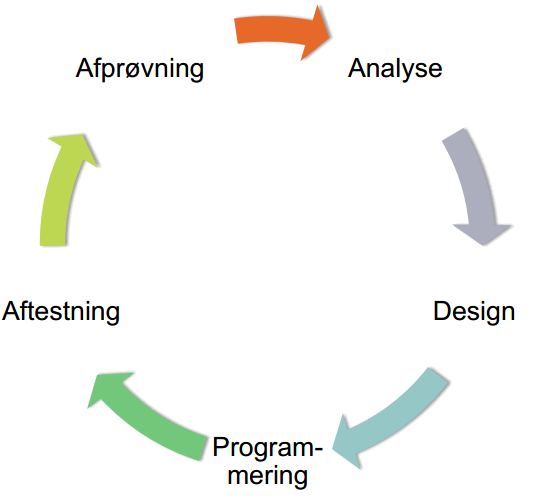
\includegraphics[scale=0.5]{billeder/evolutionaeremetode.png}
  		\capt{Figuren illustrerer en fase, i den evolutionære arbejdsmetode. En enkelt fase i udviklingsforløbet, 					  gennemgår samtlige dele af projektet.}
  		\label{fig:evolutionaeremetode}
\end{figure}

Modsat findes den konstruktive arbejdsmetode (også kaldet vandfaldsmetoden), som har en liniær tilgang til udviklingsprocessen. Den konstruktive arbejdsmetode, er også delt op i faser, men hver fase er modsat i den evolutionære metode, fokuseret henimod en specifik projektdel, se \figref{fig:konstruktivemetode}. Typisk vil et systemudviklingsforløb med udgangspunkt i den kontruktive arbejdsmetode starter ud med en analyse. Når analysen er færdig, påbegyndes design, og derefter programmering osv. Metoden bruges ofte i systemudviklingsprocesser, hvor det problem der arbejdes ud fra, er veldefineret og klart. Det er grundet, at metoden ikke, på samme måde som den evolutionære arbejdsmetode, er dynamisk, i forhold til hvis problemet ændre sig undervejs i forløbet.     

\begin{figure}[h]
		\centering
		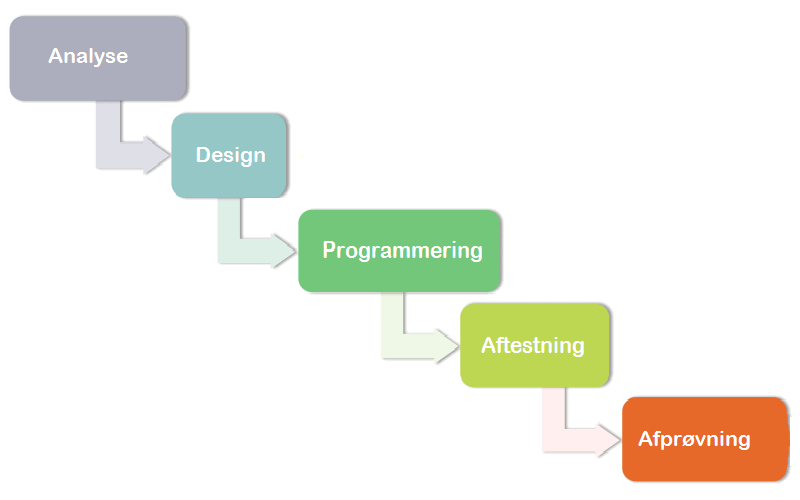
\includegraphics[scale=0.5]{billeder/konstruktivemetode.png}
  		\capt{figuren illustrerer den konstruktive arbejdsmetode.}
  		\label{fig:konstruktivemetode}
\end{figure}

Vi har kort beskrevet den evolutionære og den konstruktive arbejdsmetode. Vi har desuden beskrevet, at den evolutionære arbejdsmetode, er mere fleksibel, i forhold til den konstruktive arbejdmetode, når det problem, som skal løses, ændre sig. Men hvilke andre fordele og ulember er der, ved at vælge den ene arbejdsmetode, frem for den anden? Det kommer meget an på situationen. En forskel mellem de to metoder, er bl.a. dens måde at interagere med bruger/informanter. Mens der foregår et tæt samarbejde med informanter i den evolutionære arbejdsmetode, hvor der anvendes prototyper; har informanterne en mere passiv rolle, hvor de godkender beslutninger, og fungere som resurcer til informantion. Alt efter hvilke brguere/informanter man arbejder sammen med i sit projekt, vil den ene arbejdsmetode, være at foretrække fremfor den anden. En anden forskel mellem de to metoder, er dets tilgang til det endelig produkt/system. Den konstruktive arbejdsmetode har en meget strengent og langsigtet tidsplan, og man er ikke i tvivl om, hvornår produktet/systemet er færdigt. I en systemudviklingsproces med den evolutionære arbejdsmetodes tilgang, kan det modsat være svært, at vurdere  hvornår systemet er færdigt. Det vil altid være muligt at gå igennem endnu en iteration, og lave nye tilføjelser og redigeringer.

Der er altså store forskelle på de to arbejdsmetodes tilgang til en systemudviklingsproces, og det er derfor op til situationen, hvilken der vil fungere bedst. Det er dog væsentligt at nævne, at det næsten aldrig vil være muligt, i en udviklingsproces, udelukkende at arbejde ud fra den ene arbejdsmetode. Som regel vil elementer fra begge arbejdsmetoder, blive implementeret, men én vil være dominerende. I vores projektforløb, anvendte vi også elementer fra begge metoder, men udgangspunktet var den evolutionære arbejdsmetode. Dette var grundet, at problemet som vi fokuserede på, ikke var fuldkommen klart i den initierende del af forløbet. Vi havde kurser, sideløbende med projektet, som gjorde at vi ikke kunne komme igennem hver eneste projektdel, da vi først skulle introduceres for nogle begreber, i vores kurser omhandlende systemudvikling \cite{ooad} og designing interactive systems \cite{deb}. Vores arbejdsmetode, er illustreret i \figref{fig:blandingsmetode}. Vi delte processen op i 4 faser, hvor vi i de to første faser, udelukkende arbejdede med analyse- og designdelen. Først i tredje fase b  

\begin{figure}[h]
		\centering
		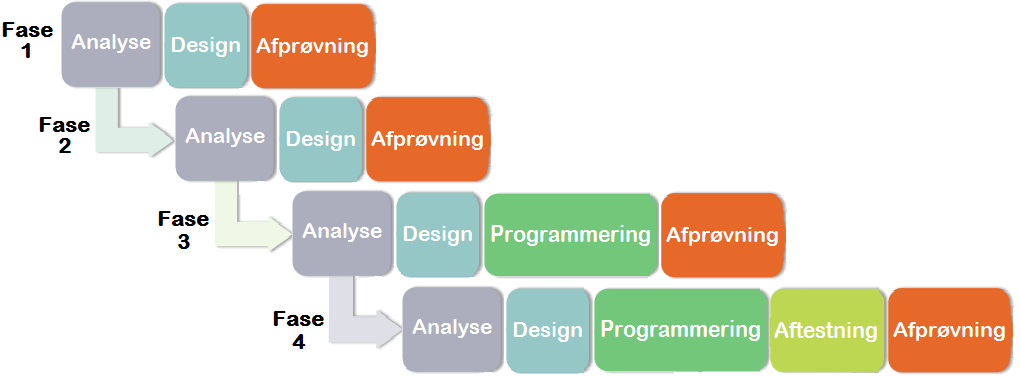
\includegraphics[scale=0.5]{billeder/blandingsmetode.png}
  		\capt{figuren illustrerer gruppens arbejdsmetode, som har været en blanding mellem den evolutionære og kostruktive arbejdsmetode.}
  		\label{fig:blandingsmetode}
\end{figure}

%% Hvordan kunne det være blevet gjort bedre i fremtidige projekter?



%% DONE:
%% konstruktive metode
%% fordele og ulember
%% Hvad har vi anvendt?